\section*{Exercice 1}
\noindent 1) \textit{Réaliser une ACP (analyse en composantes principales) sur l’ensemble des variables de la base, à l’aide du logiciel STATA, et interpréter les résultats.} \\

Après avoir effectué le test de l'ACP grâce à la commande : 
\begin{lstlisting}[style=Stata]
	pca popul tact superf nbentr nbbrev chom teleph
\end{lstlisting}

On obtient donc les résultats suivants : 61,85\% de l'inertie est expliquée par la variable \textbf{population}, tandis que la variable \textbf{taux d'activité} explique 20,42\% de l'inertie. Par ailleurs, 14,46\% de l'inertie est expliquée par la variable \textbf{superficie de la région}, 2,61\% de l'inertie est expliquée par la variable \textbf{nombre d'entreprises dans la région}, et 0,47\% de l'inertie est expliquée par la variable \textbf{nombre de brevets déposés au cours de l'année}. Enfin, les variables \textbf{taux de chômage} et \textbf{nombre de lignes téléphoniques en place dans la région} expliquent respectivement 0,15\% et 0,03\% de l'inertie.

En outre, en appliquant le critère de Kaiser, nous choisirons 3 composantes car seulement celles-ci ont des valeurs propres supérieures à 1 (4,33 ; 1,43 ; 1,02). Dès lors, $k$ sera égal à 3 au lieu de 7\footnote{Cette valeur désigne le nombre de variables}.

Concernant les valeurs des différentes composantes, nous aurons autant de composantes que de variables, dont les équations sont données comme suit :
\vspace*{-.5cm}
\[
\begin{cases}
	\text{C}^1 = 0,46 \text{Popul} + 0,35 \text{tact} - 0,01 \text{superf} + 0,46 \text{nbentr} + 0,47 \text{nbbrev} - 0,14 \text{chom} + 0,47 \text{telph}\\
		\vdots\\
	\text{C}^7 = 0,38 \text{Popul} + 0,01 \text{tact} - 0,03 \text{superf} + 0,32 \text{nbentr} + 0,16 \text{nbbrev} - 0,02 \text{chom} - 0,85 \text{telph}
\end{cases}
\]

\noindent 2)\textit{ Réaliser une ACP sur l’ensemble des variables, en permutant les positions de la première et de la deuxième variable de la base.}\\

Après avoir effectué le test de l'ACP grâce à la commande : 
\begin{lstlisting}[style=Stata]
	pca popul tact superf nbentr nbbrev chom teleph
\end{lstlisting}

On obtient donc les résultats suivants : 61,85\% de l'inertie est expliquée par la variable \textbf{taux d'activité}, tandis que la variable \textbf{population} explique 20,42\% de l'inertie. Par ailleurs, 14,46\% de l'inertie est expliquée par la variable \textbf{superficie de la région}, 2,61\% de l'inertie est expliquée par la variable \textbf{nombre d'entreprises dans la région}, et 0,47\% de l'inertie est expliquée par la variable \textbf{nombre de brevets déposés au cours de l'année}. Enfin, les variables \textbf{taux de chômage} et \textbf{nombre de lignes téléphoniques en place dans la région} expliquent respectivement 0,15\% et 0,03\% de l'inertie.

En outre, en appliquant le critère de Kaiser, nous choisirons 3 composantes car seulement celles-ci ont des valeurs propres supérieures à 1 (4,33 ; 1,43 ; 1,02). Dès lors, $k$ sera égal à 3 au lieu de 7\footnote{Cette valeur désigne le nombre de variables}.

Concernant les valeurs des différentes composantes, nous aurons autant de composantes que de variables, dont les équations sont données comme suit : \vspace*{-.5cm}
\[
\begin{cases}
	\text{C}^1 =  0,35 \text{tact} + 0,46 \text{Popul} - 0,01 \text{superf} + 0,46 \text{nbentr} + 0,47 \text{nbbrev} - 0,14 \text{chom} + 0,47 \text{telph}\\
	\vdots\\
	\text{C}^7 =  0,01 \text{tact} + 0,38 \text{Popul} - 0,03 \text{superf} + 0,32 \text{nbentr} + 0,16 \text{nbbrev} - 0,02 \text{chom} - 0,85 \text{telph}
\end{cases}
\] 

\noindent 3) \textit{Analyser les différences dans les résultats des questions 1 et 2. Commenter.} \\

Il n'existe pas de différence entre les deux estimations. Cela pourrait s'expliquer par le fait de la non existence d'une variable indépendante et dépendante dans l'Analyse des composantes principales.\\

\noindent 4) \textit{Donner la syntaxe de STATA pour présenter dans un tableau, après réalisation de l’ACP, les statistiques descriptives (moyenne, écart-type, minimum, maximum) des variables utilisées. Le nombre d’observations ne doit pas apparaitre dans le tableau.} \\

\begin{lstlisting}[style=Stata]
	summarize popul tact superf nbentr nbbrev chom teleph
\end{lstlisting}

\noindent 5) \textit{Exécuter la commande « screeplot » après réalisation de l’ACP, et interpréter le résultat obtenu.}\\

\begin{figure}[H]
	\centering 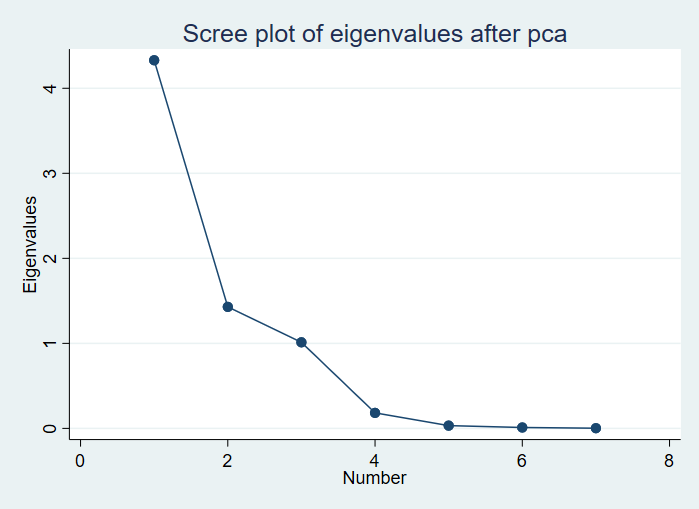
\includegraphics[width=0.6\textwidth]{C:/Users/Emmanuel/Documents/Publications/20240222 - Devoir d'analyse de données Master 1 éco/Graph.png}
	\caption{Diagramme de coude des valeurs propres après le test de l'ACP}
\end{figure}

\noindent \textbf{\underline{INTERPR\'ETATION :}} L'on constate que la variance expliquée par chaque composante principale (COMP$_i$ pour $i\in \{1;2;...;7\}$) est décroissante. Par ailleurs, contrairement aux composantes 4, 5, 6 et 7, dont ($\lambda_i<1$, pour $i\in  \{4;5;...;7\}$) les composantes principales 1, 2 et 3 apportent plus d'information que les variables principales.